% 2013_04_22_geo.tex
% 2013-04-21 dmontaner@cipf.es
% Master en Bioinformatica UV
% Nociones básicas de bioinformática y genómica

%% INTRODUCTION TO BioMart

\documentclass{beamer}
\usepackage[utf8]{inputenc}
%\usepackage[spanish]{babel}
%\usepackage[spanish,english]{babel}
\usepackage[english]{babel}

\hypersetup{colorlinks=true, citecolor=black, filecolor=black, linkcolor=blue, urlcolor=blue} %color de los links %\usepackage{hyperref} va incluido
\setbeamertemplate{frametitle}[default][center]
\setbeamertemplate{itemize items}[ball]

\graphicspath{{plots/}}

%\usepackage{enumitem}
%\usepackage{mdwlist}
%%%%%%%%%%%%%%%%%%%%%%%%%%%%%%%%%%%%%%%%%%%%%%%%%%%%%%%%%%%%%%%%%%%%%%%%%%%%%%%%

\title{BioMart}
\date{22 Aplril 2013}

\subtitle{and the Bioconductor package biomaRt}
\author{David Montaner \\ 
  %\href{http://www.dmontaner.com}{http://bioinfo.cipf.es/dmontaner} \\ 
  \href{http://www.dmontaner.es/materiales}{www.dmontaner.es/materiales} \\ 
  %\href{mailto:dmontaner@cipf.es}{dmontaner@cipf.es}}
  dmontaner@cipf.es}


%%%%%%%%%%%%%%%%%%%%%%%%%%%%%%%%%%%%%%%%%%%%%%%%%%%%%%%%%%%%%%%%%%%%%%%%%%%%%%%%
%% DOCUMENTO %%%%%%%%%%%%%%%%%%%%%%%%%%%%%%%%%%%%%%%%%%%%%%%%%%%%%%%%%%%%%%%%%%%
%%%%%%%%%%%%%%%%%%%%%%%%%%%%%%%%%%%%%%%%%%%%%%%%%%%%%%%%%%%%%%%%%%%%%%%%%%%%%%%%
\begin{document}
\begin{frame}
  \maketitle
\end{frame}

%\begin{otherlanguage}{spanish}

%%%%%%%%%%%%%%%%%%%%%%%%%%%%%%%%%%%%%%%%%%%%%%%%%%%%%%%%%%%%%%%%%%%%%%%%%%%%%%%%
%% SLIDES empiezan aqui despues del titulo %%%%%%%%%%%%%%%%%%%%%%%%%%%%%%%%%%%%%
%%%%%%%%%%%%%%%%%%%%%%%%%%%%%%%%%%%%%%%%%%%%%%%%%%%%%%%%%%%%%%%%%%%%%%%%%%%%%%%%

%\setbeamerfont*{itemize/enumerate body}{size=\footnotesize}

\begin{frame}[allowframebreaks]
  \frametitle{What is BioMart}
  
  \begin{itemize}
  \item A federated database system that provides unified access to disparate, geographically distributed data sources.
  \item Any existing databases can easily be incorporated into the BioMart framework.
  \item It is designed to be data platform independent.  
  \item Efficient. Ej. parallel query processing \dots
  \item Unified technology.
  \item No need of programming: graphical user interfaces. 
  \end{itemize}  
  
  %\bigskip
  \framebreak
  
  The BioMart project provides:
  
  \begin{itemize}
  \item software: server \dots client
  \item \textbf{services}: already set up servers that provide access to a data.
  \end{itemize}  

  \bigskip

  \centering
  \url{http://www.biomart.org/}
  
\end{frame}

%%%%%%%%%%%%%%%%%%%%%%%%%%%%%%%%%%%%%%%%%%%%%%%%%%%%%%%%%%%%%%%%%%%%%%%%%%%%%%%%

\begin{frame}
  \frametitle{BioMart Community}
  
  \begin{center}
    % \includegraphics[scale=0.3]{} 
    \href{http://central.biomart.org/}{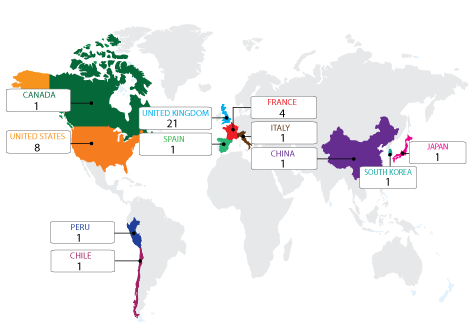
\includegraphics[width=\linewidth]{mapa}}
  \end{center}

\end{frame}

%%%%%%%%%%%%%%%%%%%%%%%%%%%%%%%%%%%%%%%%%%%%%%%%%%%%%%%%%%%%%%%%%%%%%%%%%%%%%%%%

\begin{frame}
  \frametitle{BioMart Central Portal}
  
  \begin{center}
    % \includegraphics[scale=0.3]{} 
    \href{http://central.biomart.org/}{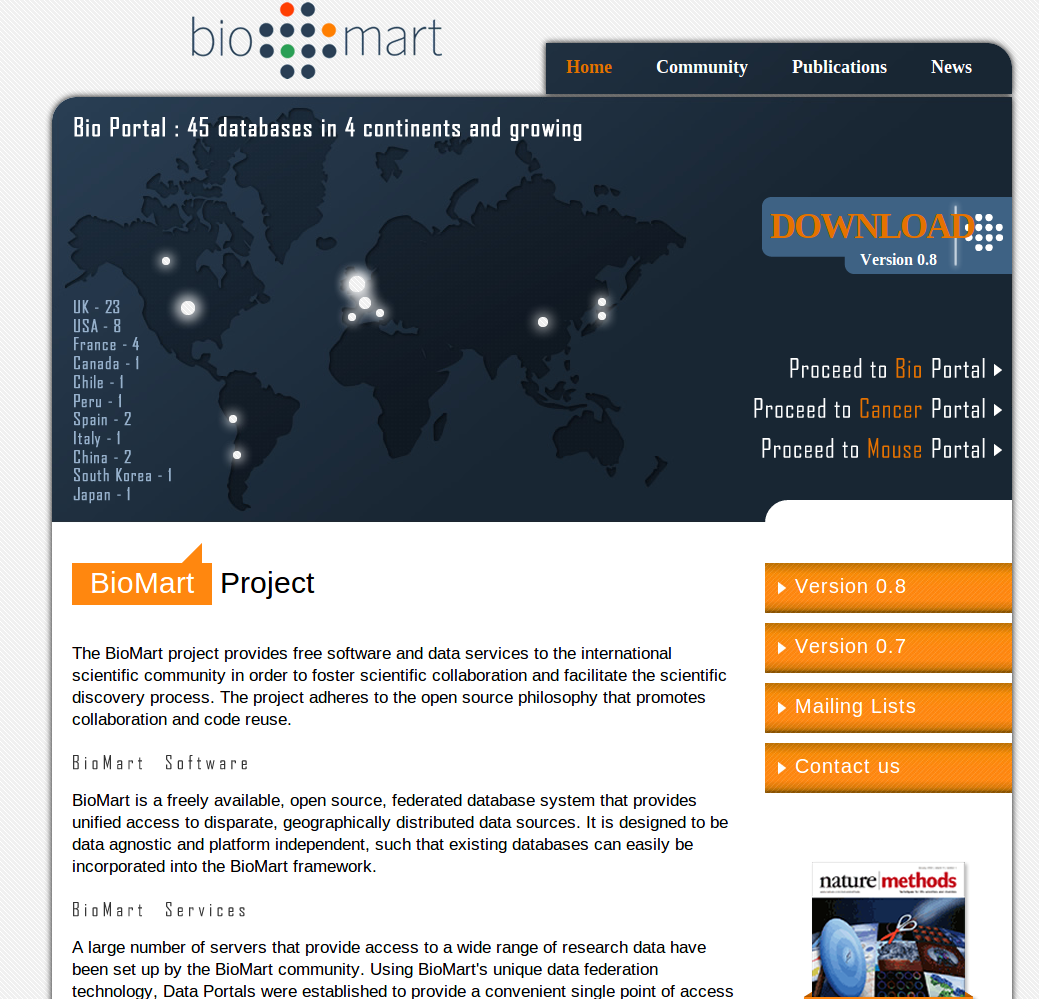
\includegraphics[width=\linewidth]{biomart_central}}
  \end{center}

\end{frame}

%%%%%%%%%%%%%%%%%%%%%%%%%%%%%%%%%%%%%%%%%%%%%%%%%%%%%%%%%%%%%%%%%%%%%%%%%%%%%%%%


\begin{frame}
  \frametitle{Standardized Access}
  \framesubtitle{(for all users)}
  
  \begin{itemize}
  \item Choose a Database. The repository.
  \item Dataset. For instance,  Species.
  \item Select Attributes: IDs, descriptions, sequences \dots \\
    Attributes are what we want to know about the genes.
  \item Set Filters. \\
    Indicate where our search should be restricted.
  \end{itemize}

  \bigskip

  Examples:
  
  \begin{itemize}
  \item \href{http://central.biomart.org/}{BioMart Central Portal}
  \item \href{http://www.ensembl.org/biomart/martview/857f918a2fae8d24602f998adfda2ef8}{EnsMart} form Ensembl.
  \item \href{http://hapmap.ncbi.nlm.nih.gov/biomart/martview/767d14a9a8473f2b6264357cd5afe8d8}{HapMap}.
  \item \href{http://caprica.caltech.edu:9002/biomart/martview/35a1d0dd0809f32472ff59325d39456e}{WormBase}
  \item \href{http://biomart.intogen.org/biomart/martview/b2abea454025567d06f7112de64c29b5}{IntOGen} Spanish.
  \end{itemize}

\end{frame}

%%%%%%%%%%%%%%%%%%%%%%%%%%%%%%%%%%%%%%%%%%%%%%%%%%%%%%%%%%%%%%%%%%%%%%%%%%%%%%%%

\begin{frame}
  \frametitle{biomaRt}

  \url{http://www.bioconductor.org/packages/release/bioc/html/biomaRt.html}

\end{frame}  

%%%%%%%%%%%%%%%%%%%%%%%%%%%%%%%%%%%%%%%%%%%%%%%%%%%%%%%%%%%%%%%%%%%%%%%%%%%%%%%%

\begin{frame}
  \frametitle{References}

  \begin{itemize}
  \item \url{http://www.biomart.org/}
  \item \url{http://www.bioconductor.org}
  \end{itemize}

\end{frame}  

% %% FIN DOCUMENTO %%%%%%%%%%%%%%%%%%%%%%%%%%%%%%%%%%%%%%%%%%%%%%%%%%%%%%%%%%%%%%%
\end{document}
